%
% $RCSfile: software_engineering_process.tex,v $
%
% Copyright (c) 2001-2004. Christian Heller. All rights reserved.
%
% No copying, altering, distribution or any other actions concerning this
% document, except after explicit permission by the author!
% At some later point in time, this document is planned to be put under
% the GNU FDL license. For now, _everything_ is _restricted_ by the author.
%
% http://www.cybop.net
% - Cybernetics Oriented Programming -
%
% http://www.resmedicinae.org
% - Information in Medicine -
%
% @author Christian Heller <christian.heller@tuxtax.de>
%

\section{Software Engineering Process}
\label{software_engineering_process_heading}

For a great part, the aforementioned problems are caused by multiple \emph{Gaps}
in abstraction, that occure during a software project's lifetime. Software does
not only contain and process \emph{Information}, it is information itself.
It stands at the end of a sequence of abstractions which is called a
\emph{Software Engineering Process} (SEP). Software development history has shown
plenty of different forms of such processes, but most can be categorized into one
of the following: \emph{Waterfall Process}, \emph{Iterative Process},
\emph{Extreme Programming} (\emph{Cathedral} or \emph{Bazaar} mode),
\emph{Agile Software Development}.

This work is not exactly about software engineering processes, nor does it want
to introduce yet another one. Its main purpose is to deal with the \emph{Results}
of software development phases: \emph{Abstractions}. Probably every project goes
through the three common phases \emph{Analysis}, \emph{Design} and
\emph{Implementation} (figure \ref{knowledge_abstraction_figure}). Each of them
creates its own model of what is to be abstracted in software:

\begin{figure}[ht]
    \begin{center}
        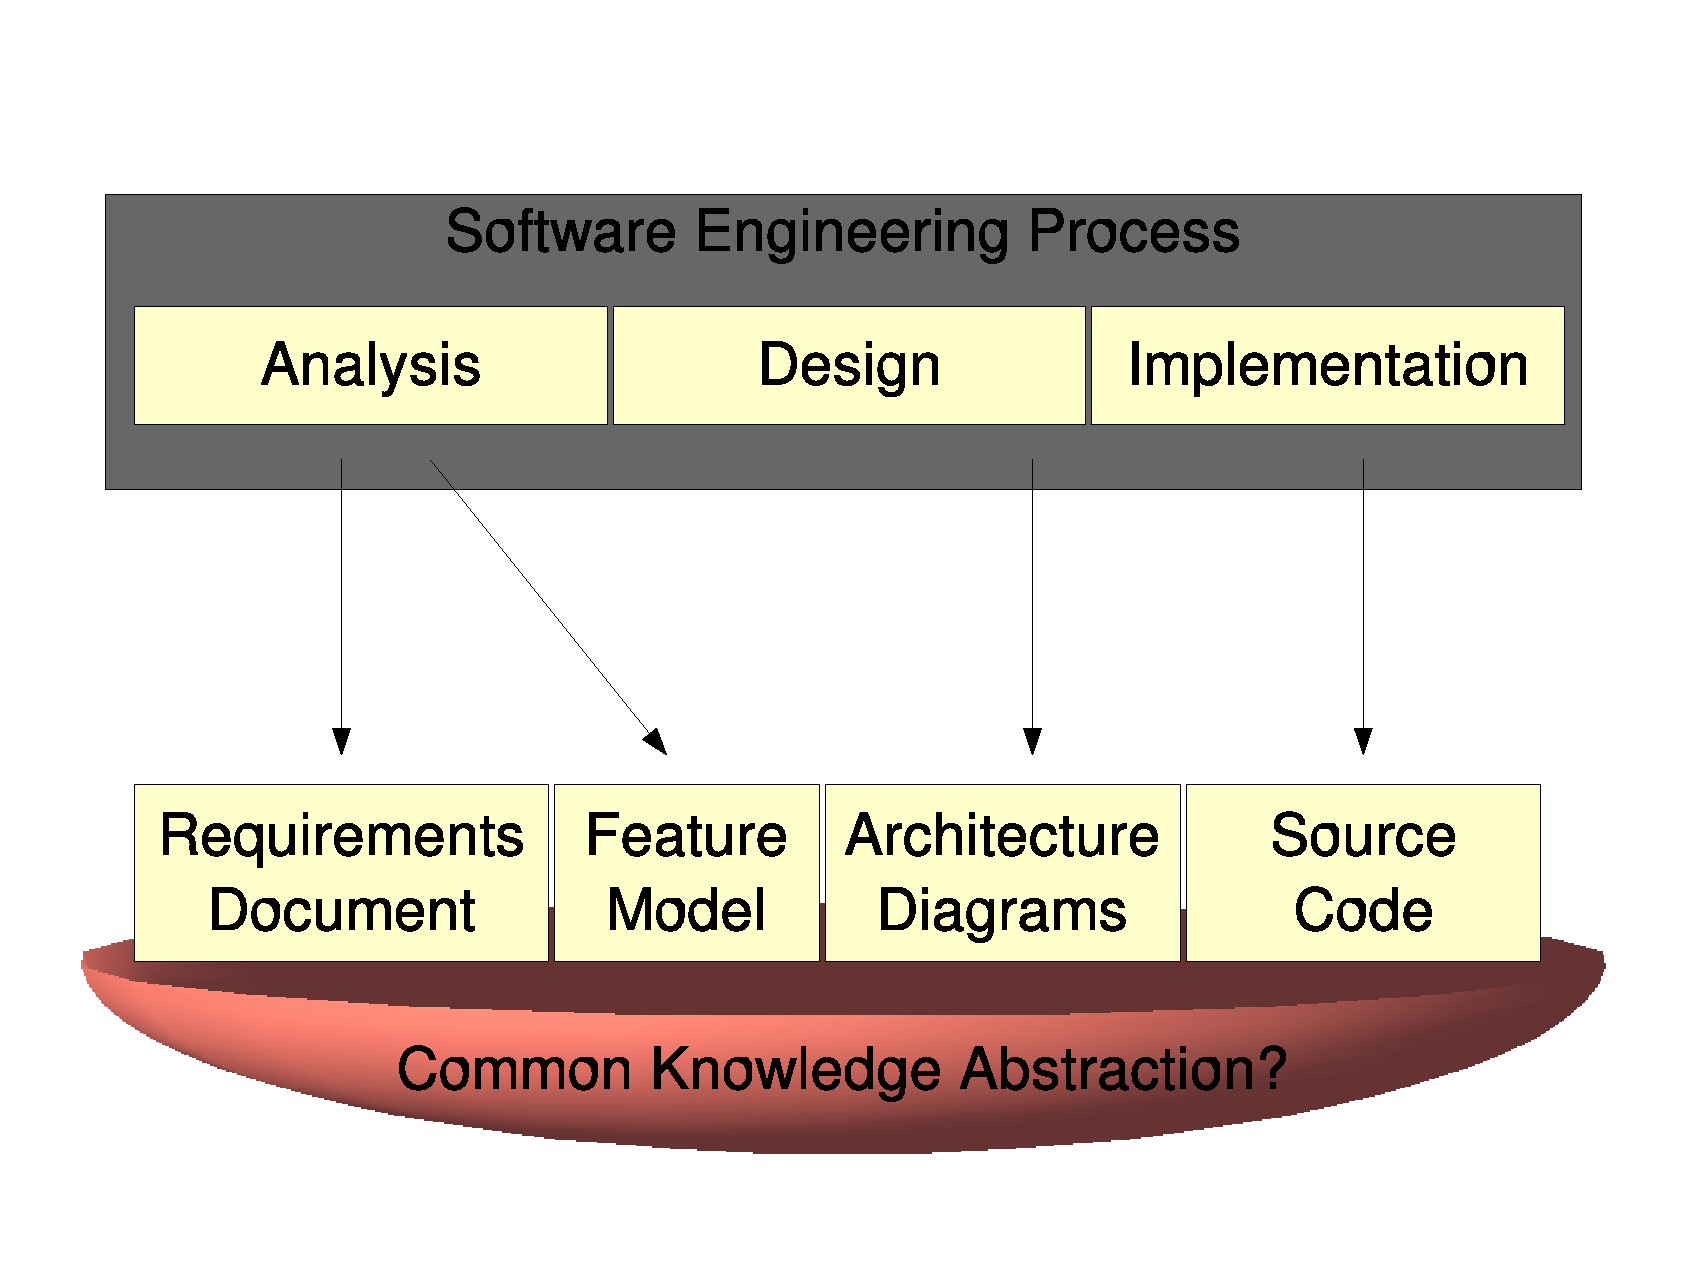
\includegraphics[scale=0.3]{vector/knowledge_abstraction.eps}
        \caption{Knowledge Abstraction}
        \label{knowledge_abstraction_figure}
    \end{center}
\end{figure}

The analysis often results in a \emph{Requirements Document} which investigates
the problem domain and uses expert knowledge to specify the functionality of the
software to be created. This specification is mostly \emph{informal}, that is an
ordered collection of textual descriptions. Sometimes, \emph{semi-formal}
descriptions such as tables or graphics are used additionally.

It is the aim of the design phase to deliver a clear system architecture with
little redundancies and only few interdependencies, which it may specify by help
of \emph{semi-formal} \emph{Diagrams}. Recent years showed an increased use of the
\emph{Unified Modelling Language} (UML), a collection of diagram specifications
for representing static or dynamic aspects of a system to be modelled.
Normally, a \emph{top-down} approach is chosen for the design of a system.
Hereby, the overall architecture is considered first, before moving into details.
The less common \emph{bottom-up} design would start the other way and first try
to build small components to construct the whole system from.

Finally, implementation of a system is done \emph{formally}, in one (or more)
programming languages. The retrieved \emph{Source Code} represents the final
abstraction, the software that was to be built.

It is obvious that at least two gaps have to be crossed when using the described
phases:

\begin{enumerate}
    \item{Requirements Document -- Architecture Diagrams}
    \item{Architecture Diagrams -- Source Code}
\end{enumerate}

Many efforts try to minimize the first gap by telling their analysis experts
to specify use cases, workflows and static structures using the corresponding
diagrams provided by the \emph{Unified Modelling Language}.
Other efforts introduce more steps of abstraction, like the \emph{Feature Model}.
It provides a hierarchical model of the features of the system to be built.
The feature analysis is part of the analysis but can logically be placed between
analysis and design. It became especially popular in the area of
\emph{System Family/ Product Line Engineering}. Yet the disadvantage of using
feature models is that another gap in abstraction is created:

\begin{enumerate}
    \item{Requirements Document -- Feature Model}
    \item{Feature Model -- Architecture Diagrams}
    \item{Architecture Diagrams -- Source Code}
\end{enumerate}

One aim of the work described in this document was to overcome these gaps by
supplying one kind of abstracted knowledge, for statics as well as for dynamics,
to be continuously used throughout all project phases.
